\documentclass{article}

% if you need to pass options to natbib, use, e.g.:
%     \PassOptionsToPackage{numbers, compress}{natbib}
% before loading neurips_2018

% ready for submission
% \usepackage{neurips_2018}

% to compile a preprint version, e.g., for submission to arXiv, add add the
% [preprint] option:
%     \usepackage[preprint]{neurips_2018}

% to compile a camera-ready version, add the [final] option, e.g.:
     \usepackage[final]{neurips_2018}

% to avoid loading the natbib package, add option nonatbib:
 %   \usepackage[nonatbib]{neurips_2018}

\usepackage[utf8]{inputenc} % allow utf-8 input
\usepackage[T1]{fontenc}    % use 8-bit T1 fonts
\usepackage{hyperref}       % hyperlinks
\usepackage{url}            % simple URL typesetting
\usepackage{booktabs}       % professional-quality tables
\usepackage{amsfonts}       % blackboard math symbols
\usepackage{nicefrac}       % compact symbols for 1/2, etc.
\usepackage{microtype}      % microtypography
\usepackage{graphicx}
\usepackage{indentfirst}
\setlength{\parindent}{2em}
\usepackage{setspace}
\usepackage {subcaption}
\usepackage{float}
\usepackage{titlesec}
\titlespacing{\section} {10pt}{3.5ex plus 1ex minus .2ex}{2.3ex plus .2ex}
\titlespacing{\chapter} {0pt}{50pt}{40pt}
%\titlespacing{\paragraph} {0pt}{3.25ex plus 1ex minus .2ex}{1em}
%\titlespacing{\subparagraph} {parindent}{3.25ex plus 1ex minus .2ex}{1em}
%\titlespacing{\subsection}{0pt}{3.25ex plus 1ex minus .2ex}{1.5ex plus .2ex}
%\setlength\textfloatsep{10bp}
%\setlength\intextsep{10bp}
%\usepackage{subfigure}

\title{Quora Insincere Question Selection}
 
% The \author macro works with any number of authors. There are two commands
% used to separate the names and addresses of multiple authors: \And and \AND.
%
% Using \And between authors leaves it to LaTeX to determine where to break the
% lines. Using \AND forces a line break at that point. So, if LaTeX puts 3 of 4
% authors names on the first line, and the last on the second line, try using
% \AND instead of \And before the third author name.

\author{%
  Peihong Yu\quad  Xinru Zhang\quad Mengjie Min\\
  Stevens Institute Of Technology\\
  \texttt{pyu7@stevens.edu\quad
  	xzhan63@stevens.edu\quad
  	mmin@stevens.edu} \\
  % examples of more authors
  % \And
  % Coauthor \\
  % Affiliation \\
  % Address \\
  % \texttt{email} \\
  % \AND
  % Coauthor \\
  % Affiliation \\
  % Address \\
  % \texttt{email} \\
  % \And
  % Coauthor \\
  % Affiliation \\
  % Address \\
  % \texttt{email} \\
  % \And
  % Coauthor \\
  % Affiliation \\
  % Address \\
  % \texttt{email} \\
}

\begin{document}
% \nipsfinalcopy is no longer used

\maketitle
\begin{abstract}
	In this Kaggle competition, we aim at finding out inappropriate questions from Quora website by building a binary classification model. We separate our whole work into three steps. First, with a deep look into the dataset, we clean the data by removing typos and filling missing data. Second, we train three different models to make our predictions. The approaches we adopt to solve the problem are "GRU", "LSTM" and "Soft Attention". Finally, submitting our predictions to kaggle and get our accuracy. Submissions are evaluated on F1 score between the predicted and the observed targets.  Owing to the incorrect labels in datasets, the highest score on the leader board in this competition is about 0.71. Our highest result reaches 0.685 which rank top 25\% in the competition. At this time, we only use one word embeddings among applied four embeddings, hoping by combining all the embeddings together can we get a better result in the future.\\
\end{abstract}
\setlength{\parskip}{0.3em}
\section{Introduction}
\noindent Quora is a website for people to communicate with others. But sometimes inappropriate questions and comments appear. Till now, the Quora has already implemented machine learning and hand-operated ways to decrease the possibility of insincere questions. In order to combat insincere questions more efficiency and help Quora maintain their policy with "Be Nice, Be Respectful", we need to find more up-gradable ways to discover these ambiguous and confusing questions.\\

\noindent The training dataset consists of three parts: id(numbers), question text(string), label(0 or 1) whereas test data lacking labels. By filling missing data, removing or replacing typos in an appropriate way, we can obtain a better result. Notice from the original data set, there are many disturbing characters. For the data pre-processing part, we majorly take four steps to clean the original data: \\

\indent1) Obtain a vocabulary by loading words from word embedding(wiki-news-300d-1M.vec). \\
\indent2) Get and analyze words in training data which are uncovered by "wiki" vocabulary.\\
\indent3) Discard the punctuation, spaces and replace the misspell words into correct spell words.\\
\indent4) Choose appropriate words in "wiki" vocabulary and replace the “cannot find” words with them.\\


\noindent Model building base on the organizer's command, we need to build a classifier to find out insincere questions. Dealing with the relationship with language, RNN is the general model we first think  to build our model. So our approaches are motivated by the success of RNN model in natural language processing field. Firstly, we  use LSTM model, which is an improvement model of RNN. The LSTM model has the ability to "remember" some information in the past and keep them to future calculations, not like general RNN model will lose those information instead. We also introduce GRU to build our model. Compared to LSTM, the commonality is that two models both keep the important information. The difference is GRU model has fewer parameters than LSTM model, so the training speed is faster. Furthermore, we adopt and adjust attention model to make predictions because we not only want our model to "remember" some past info but also focus on some potential words which may play a decisive role in sentences.\\

\noindent In principle, by submitting results to kaggle, the highest score we got is 0.68506 and have a rank at 1050 among total 4037 groups , which is quite high at this point since the original dataset contains many wrong labels. \\

\section{ Data Pre-processing}
\noindent The first and most important part of our project is data preprocessing.  We print the shape of training dataset and testing dataset on the first hand. In figure 1, the output shows that we have about 1306122 rows and 3 columns of data. The file train.csv has three columns: qid, question\_text, target. "qid" contains ids for every sentences which is useless for us.  “Question\_text” column is composed of sentences that we need to analysis and feed into our models. “Target” column has binary values. “1” means that this sentence is identified as insincere. \\
\begin{figure}[H] %1
%	\setlength{\abovecaptionskip}{0.cm}
%	\setlength{\belowcaptionskip}{-0.cm}
 	\vspace{-0.8cm}
	\centering
	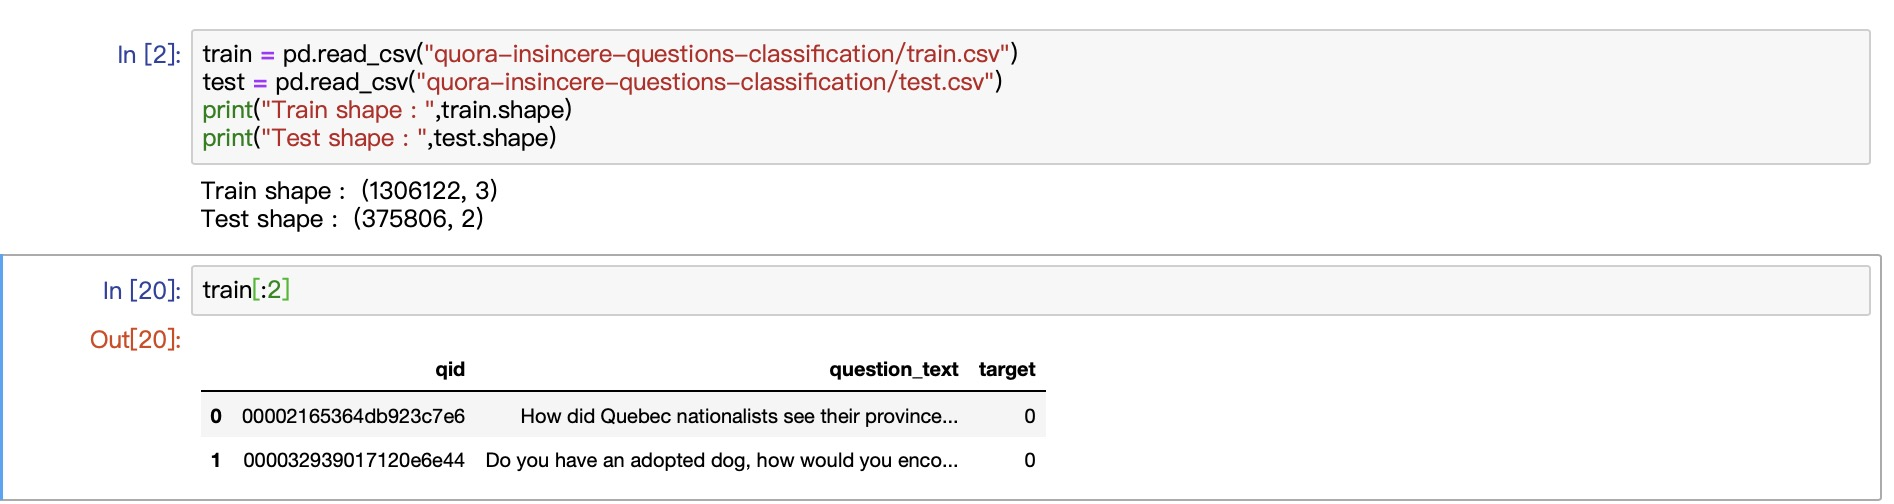
\includegraphics[scale = 0.3]{n1.jpeg}
	\caption{Information of training dataset
		}
\end{figure}
\noindent By thoroughly looking at questions, we find two problems, one is the lengths of questions are not same, the other one is typos and new words may not appear in word embedding.\\

\noindent We generate two distributions of question text length in words and characters shown as Fig 2 below. The shapes of these two distributions are very similar. In order to decide how long should we set the model’s input, we then calculate the average length and max length in Fig 3.\\
\begin{figure}[H] %2
\hspace*{0pt}
	\centering
	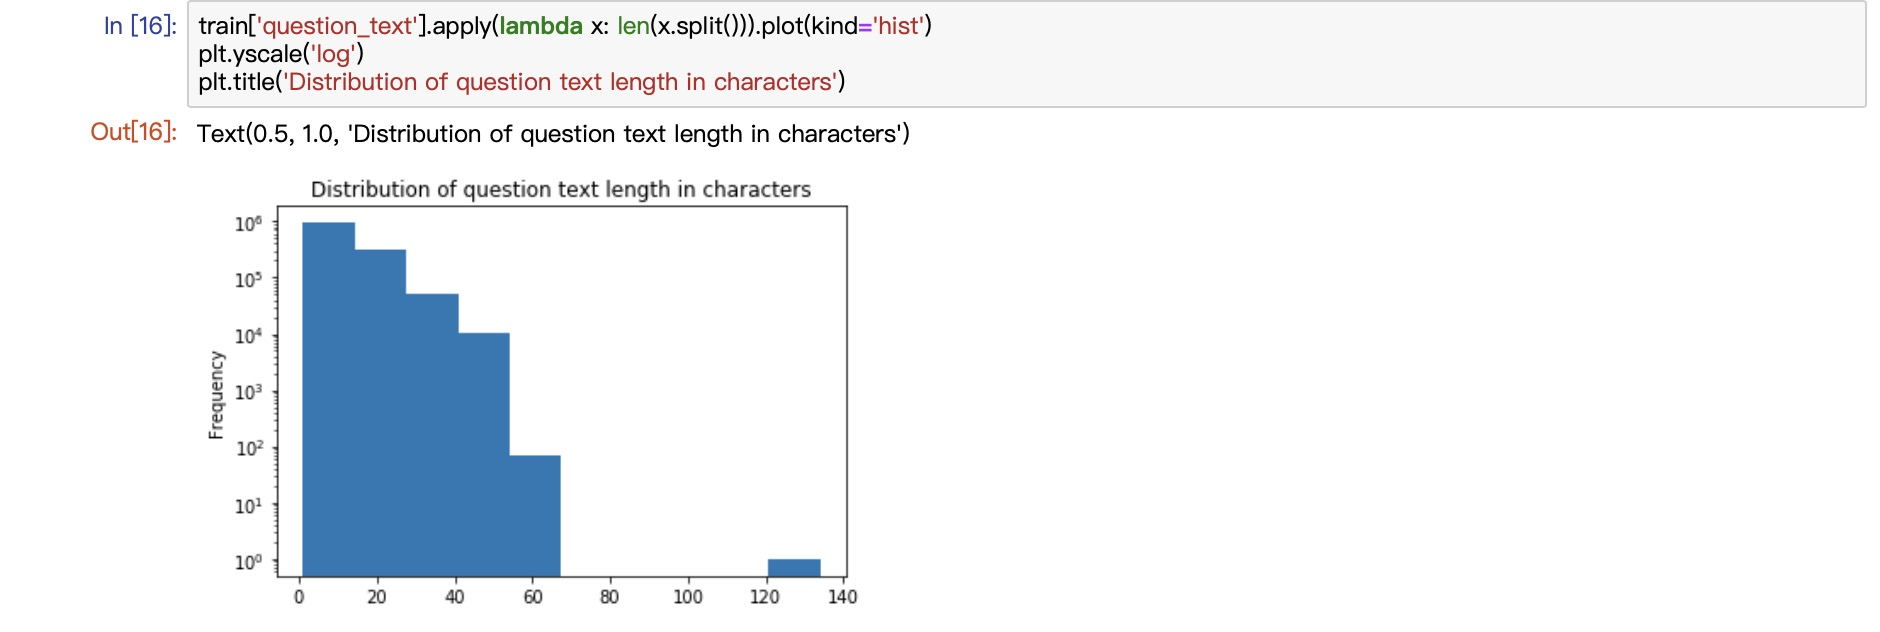
\includegraphics[scale = 0.2]{n3.jpeg}
	\caption{ Distribution of question text length in characters}
\hspace*{0pt}
\end{figure}
\begin{figure}[H]
	\centering
	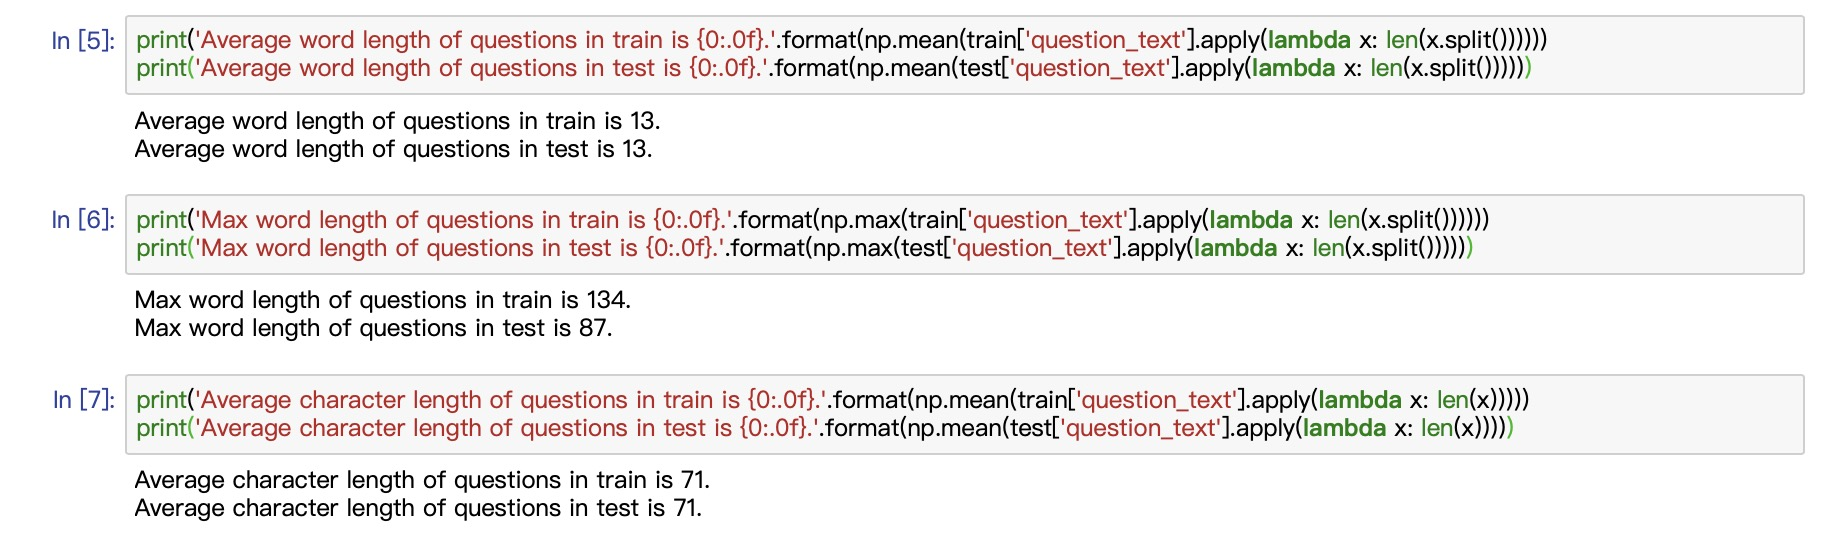
\includegraphics[scale = 0.2]{n2.jpeg} %3
	\caption{Average length and max length of questions in training dataset and testing dataset}
\end{figure}
\noindent In the result above, the average character length in train and test are all 71, so we decide to set the maximum length of words in each sentence to 72.\\

\noindent For the purpose of dealing with typos and new words, the first thing we need to do is getting vocabularies for dataset and word embedding. To get the vocabulary for dataset, we build a function called build\_vocab to collect not only words but also frequencies (Fig 4). To get the vocabulary for word embedding, we simply load from “wiki-news-300d-1M.vec” (Fig 5).\\
\begin{figure}[H]
	\centering
	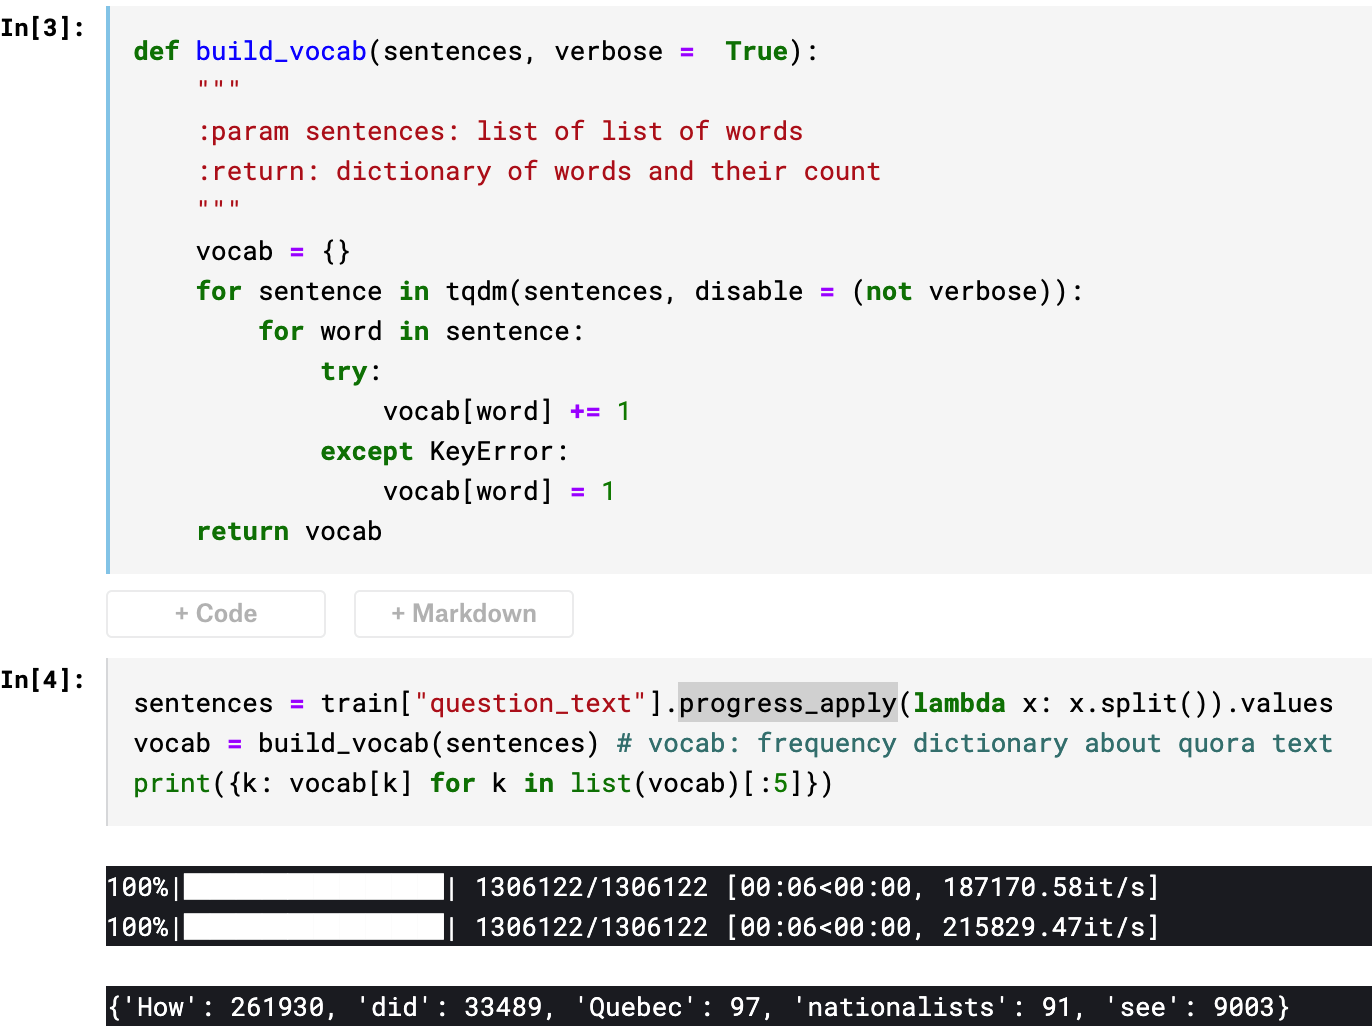
\includegraphics[scale = 0.15]{1.png} %4
	\caption{Collect words and words frequency from training dataset }
\end{figure}
\begin{figure}[H]
	\centering
	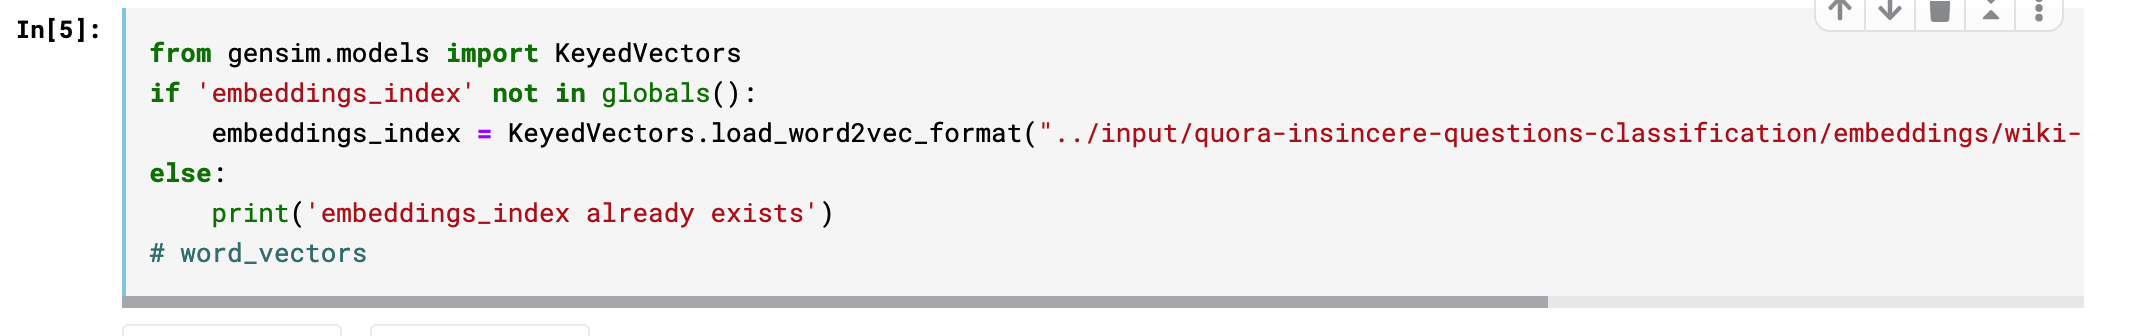
\includegraphics[scale = 0.15]{2.png} %5
	\caption{Use KeyedVectors library to change words into one-dimensional vector}
\end{figure}

\noindent By using the check\_coverage function we build, we get the uncovered sorted vocabulary called "oov" (Fig 6). Fig 7 displays top 10 uncovered words, most of them are abbreviations and words with punctuations. After manually create a misspell dictionary containing abbreviations and common misspell words with their correct format (Fig 8), we simply remove other punctuations considering punctuations may not be very useful for classification (Fig 9). What's more, we also pick 1000 words from "oov" and compare each word among sentences in the training dataset to get the according index, label and frequency. (Fig.10)\\

\begin{figure}[H]
	\centering
	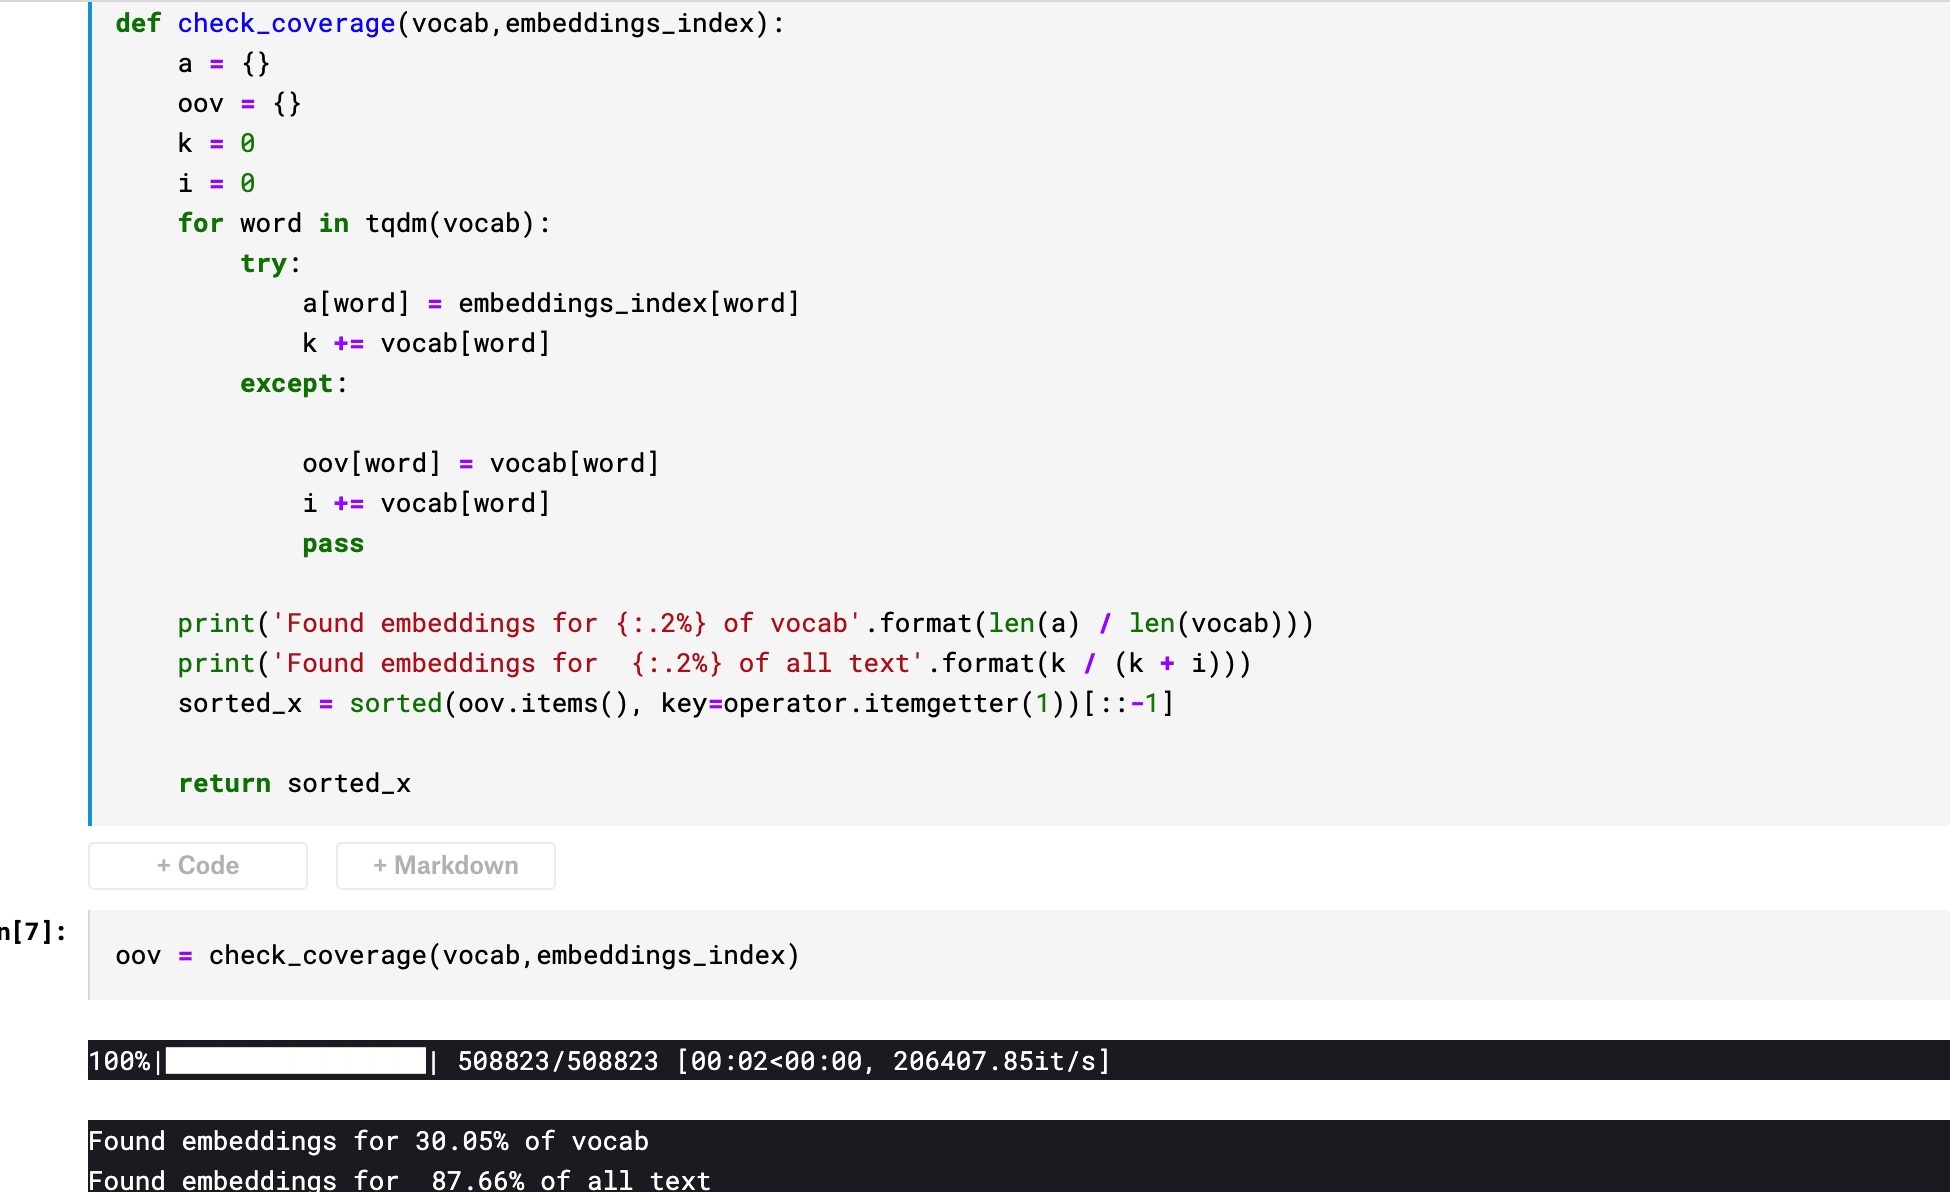
\includegraphics[scale = 0.15]{3.png} %6
	\caption{Percentage of covered and uncovered words compare to the "wiki" dataset}
\end{figure}
\begin{figure}[H]
	\centering
	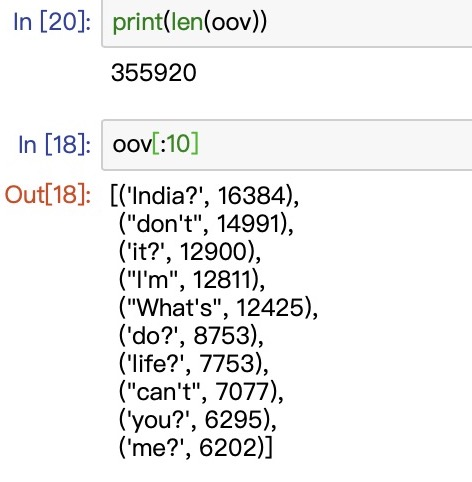
\includegraphics[scale = 0.2]{4.jpeg} %7
	\caption{Display top 10 frequency of uncovered words}
\end{figure}
\begin{figure}[H] %8
	\centering
	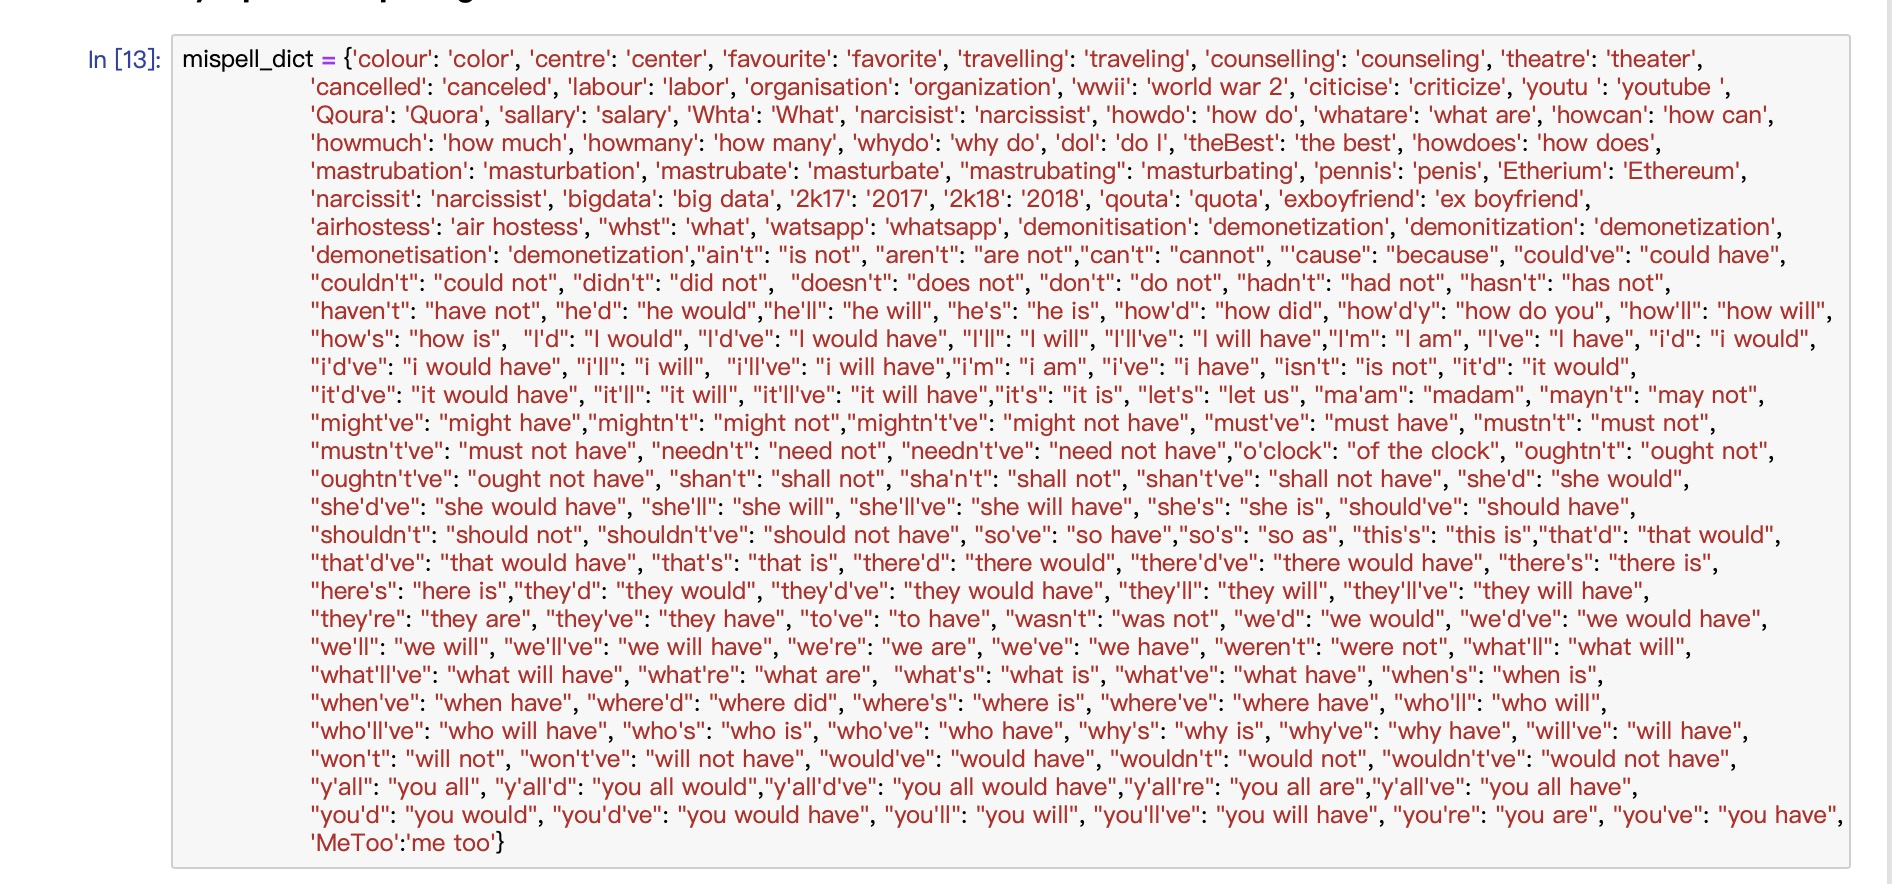
\includegraphics[scale = 0.15]{mis.jpeg} % new 8
	\caption{Manually create a misspell dictionary}
\end{figure}
\begin{figure}[H]
	\centering
	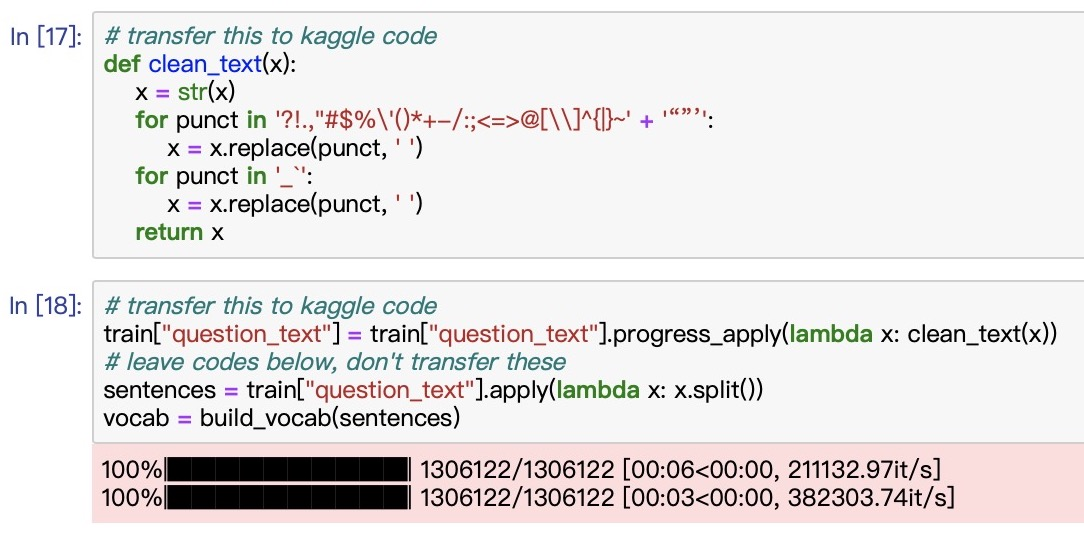
\includegraphics[scale = 0.15]{6.jpeg} %9
	\caption{Split and replace punctuations}
\end{figure}
\begin{figure}[H]
	\centering
	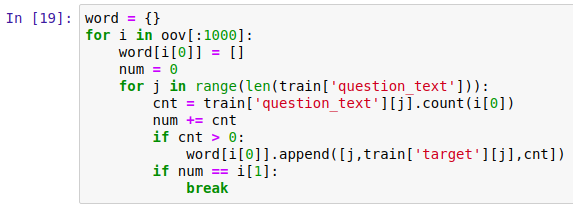
\includegraphics[scale = 0.3]{105.png} %9
	\caption{Generate mistake embedding dictionary}
\end{figure}
\noindent When we ruled out the possibility of mistyping, the number of cannot-find-word remains high which may still affect the accuracy of our model. To eliminate this effect as much as possible, we come up with a method which replaces cannot-find-word with other words based on labels. We first sort the cannot-find-word with frequencies, and then choose the top 1000 separately and count how many times they appear in good\_sentence(label 0) and bad\_sentence(label 1) in train dataset as shown in Fig 11. And calculate the ratio=bad\_times/total times (shown in Fig 12).
\begin{figure}[H]
	\centering
	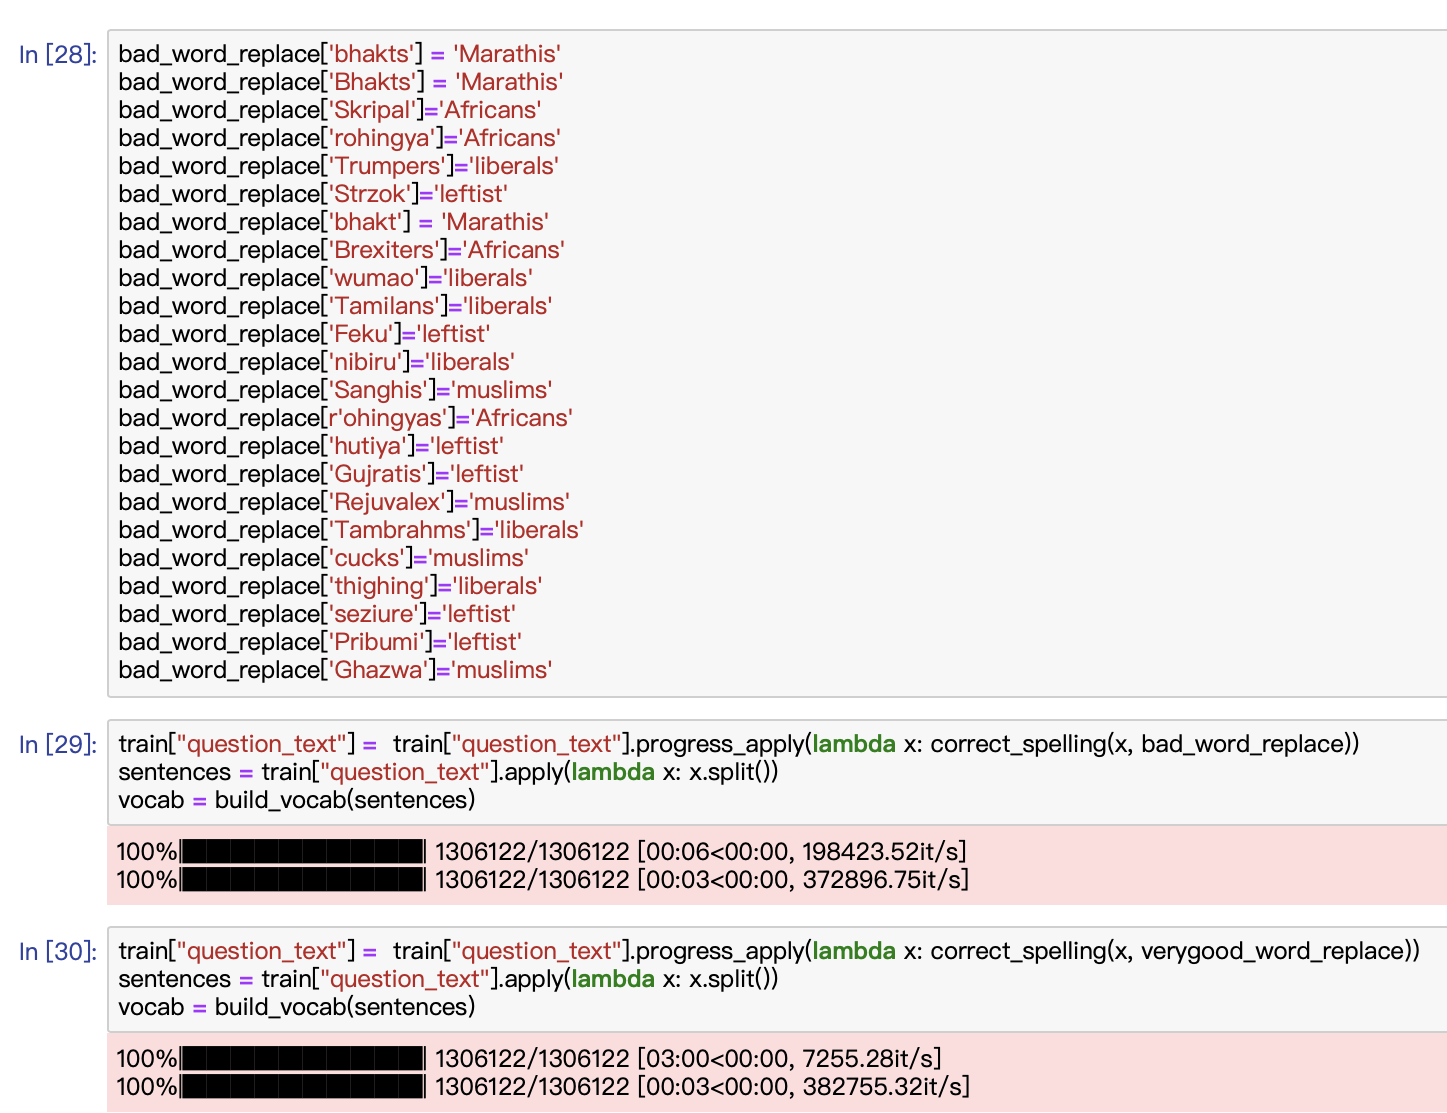
\includegraphics[scale = 0.3]{last.png} %9
	\caption{Replace cannot-find-word with other words base on labels}
\end{figure}
\begin{figure}[H] %10
	\centering
	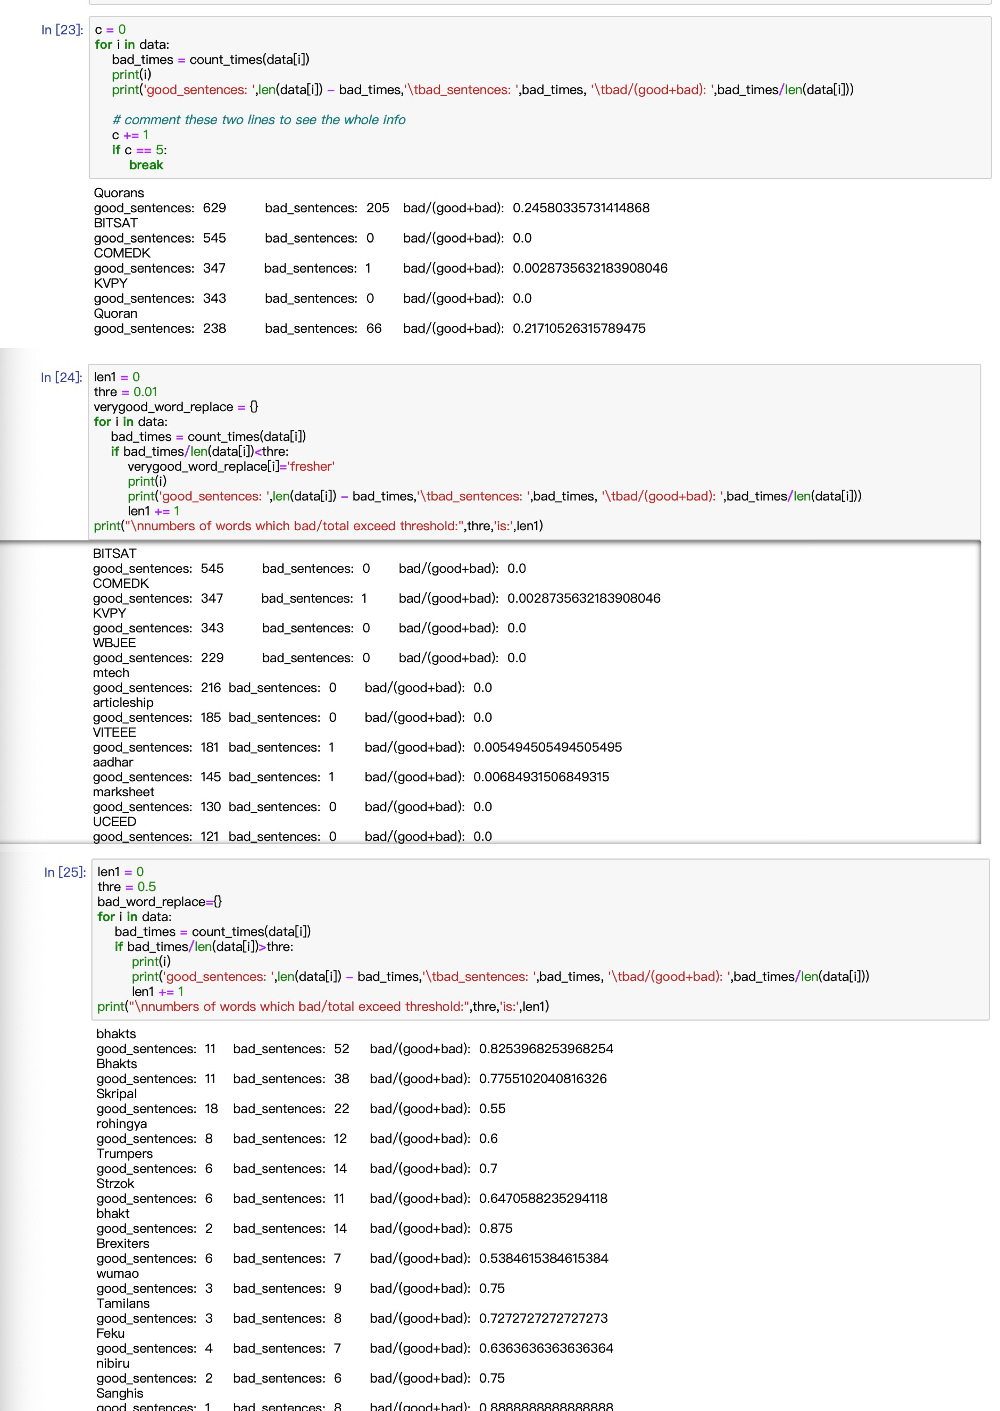
\includegraphics[scale = 0.2]{insert.jpeg}
	\caption{Calculate bad ratio of sentences within the total training dataset}
\end{figure}
\noindent At the same time, we randomly sample 1000 sentences respectively from good\_sentence and bad\_sentence. Collect words appear in these 2000 sentences and count times they appear in good\_sentence(label 0) and bad\_sentence(label 1) in train dataset. Then calculate the ratio of each word, shown in Fig 13. By setting the threshold of ratio, we can choose appropriate word with similar ratio as canno-find-word, we can replace cannot-find-word with them. For example, in Fig 13 the ratio of ‘bhakts’ is about 0.8254, and the word ‘Marathis’ has similar ratio value. As to this situation, it is theoretically feasible to replace ‘bhakts’ with ‘Marathis’\\
\begin{figure}[H] %10
	\centering
	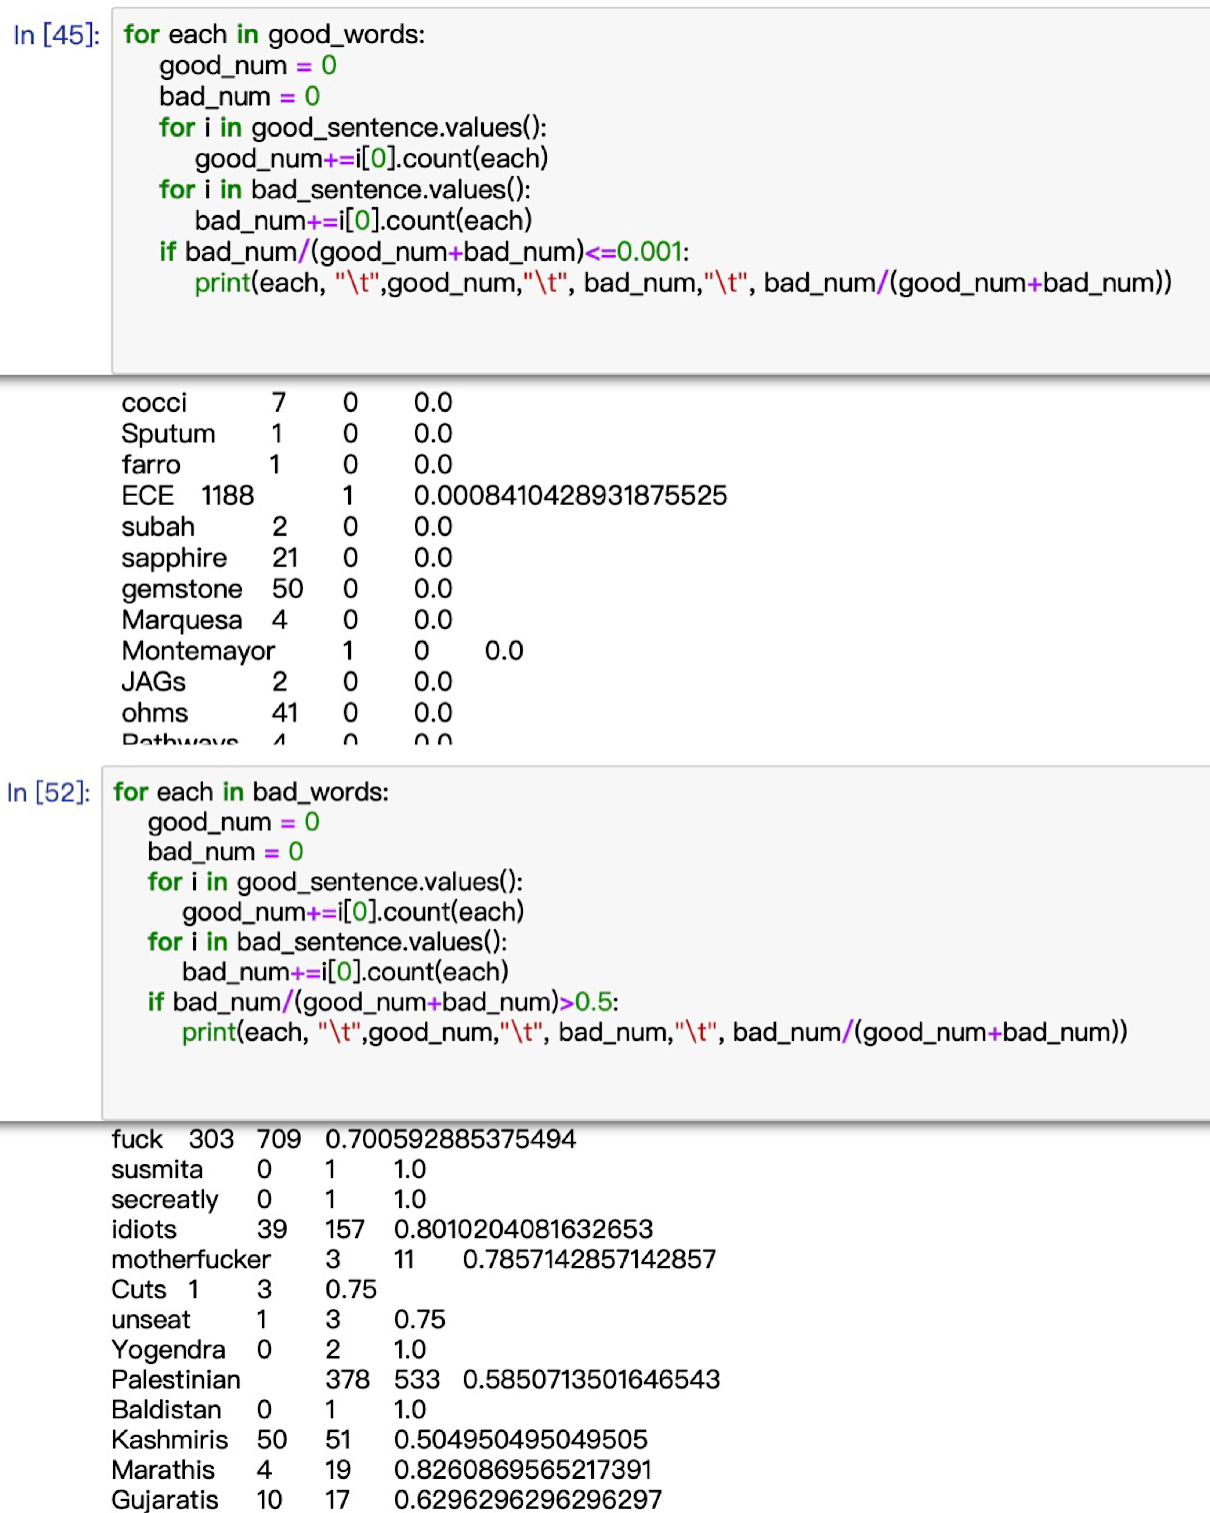
\includegraphics[scale = 0.15]{gb.jpeg}
	\caption{Calculate bad ratio of sentences within the total training dataset}
\end{figure}
\noindent After all the above process are done, we successfully reduced the number of cannot-find-word from 355920 to 79883.\\
\begin{figure}[H] %10
	\centering
	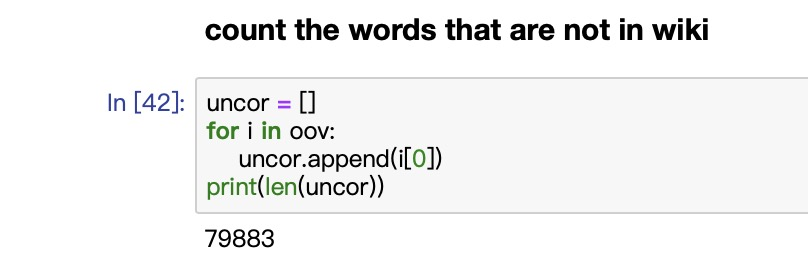
\includegraphics[scale = 0.2]{79883.jpeg}
	\caption{The list length changes from 355920 to 79883}
\end{figure}





\section{ Model Selection}
\noindent In deep learning when we talk about text classification,
the first and most popular model appears in our mind must be RNN model. As we read a sentence, we will not restart from the beginning of the sentence when we meet a new word. Our brain will comprehension from words we have already read and infer the meaning of new words. At this time, our own modules are inspired by Vanilla RNN, LSTM and GRU these three modules. Besides we also make stack and combination from three modules above.
\subsection{Vanilla RNN}
\noindent Recurrent neural networks is not a new topic in deep learning area. Many famous network company as Baidu, Google extensively use this technique with machine translation, speech recognition as well as a number of other tasks. Especially, almost all state of the art outcomes in NLP related tasks are achieved by exploiting RNNs. Before RNN, traditional neuron networks cannot contain persistance, it seems like a corrupt practices. But the occurrence of RNN solve this problem.
\begin{figure}[H]
	\centering
	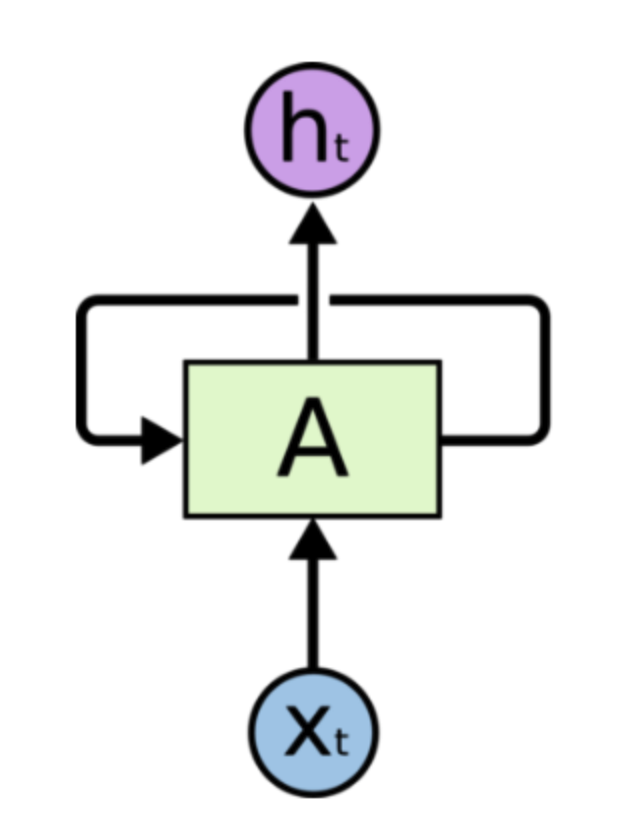
\includegraphics[scale = 0.15]{7.png}
	\caption{Single recurrent neural network model}
\end{figure}
\noindent The recurrent neural networks model is in Fig.15 above. During each time period, each node receives information from the previous node and the process can be represented by a feedback cycle. Fig.16 shows the details of this "feedback" cycle.
\begin{figure}[h]
	\centering
	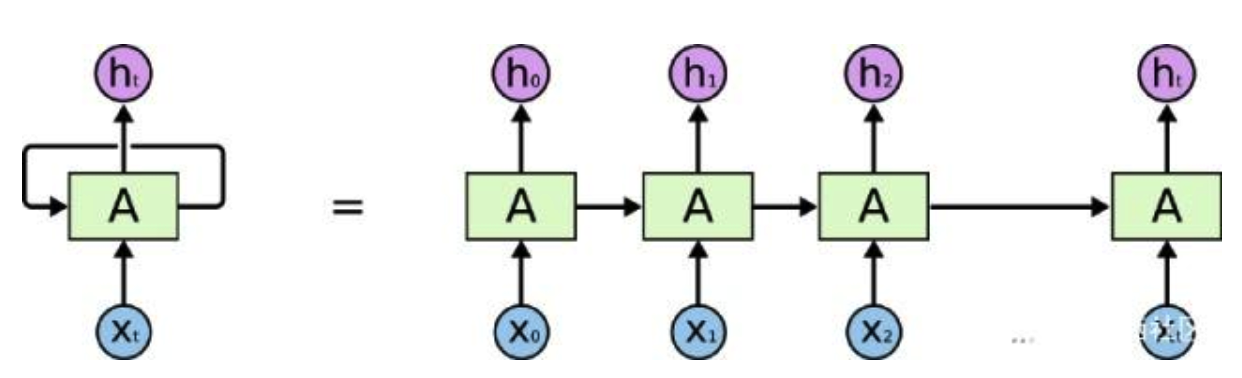
\includegraphics[scale = 0.2]{8.png}
	\caption{How recurrent neural network work}
\end{figure}\\
\noindent In each time process, we pick an input " xi " and output of previous node "ai - 1". Calculate them and get the output of the current node " hi ". Same, the output "hi" also provided to the next node as it's input. The cycle will continue running until all time process finish.\\

\subsection{LSTM}
\noindent The defect of RNN is that with the growth of time period, it cannot get effect information from the time period a long time before. If we want to know more information with "t+1", we probably need to realize the meaning from "0" and "1" in the time process. Due to the long distance, the model learns from "0" and "1" cannot be expressed to the node with " t+1 ". As far as we can see, RNN can only memorize the short information sequence.
\begin{figure}[h]
	\centering
	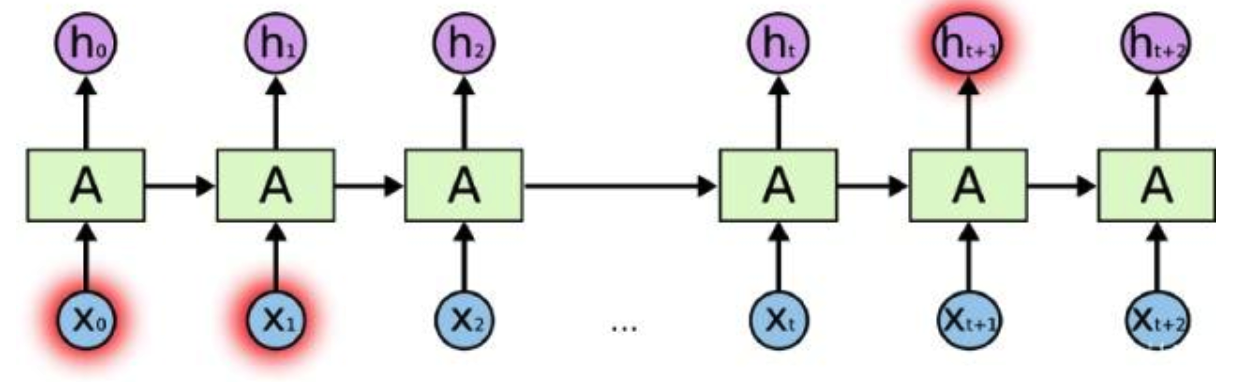
\includegraphics[scale = 0.15]{9.png}
	\caption{RNN cannot get information with long period before}
\end{figure}\\
\noindent As a result LSTM networks came. LSTM is not a totally new module, it's a kind of evolution from RNN module. In order to keep and transfer information for a long period of time is the default behavior of these networks. Comparing with the structure, both LSTM and RNNs have a chain like shape. But the repeating module from two models are quite different. The original repeating module of RNNs only has a single tanh layer, but LSTM module contains four interacting layers.
\begin{figure}[H]
	\centering
	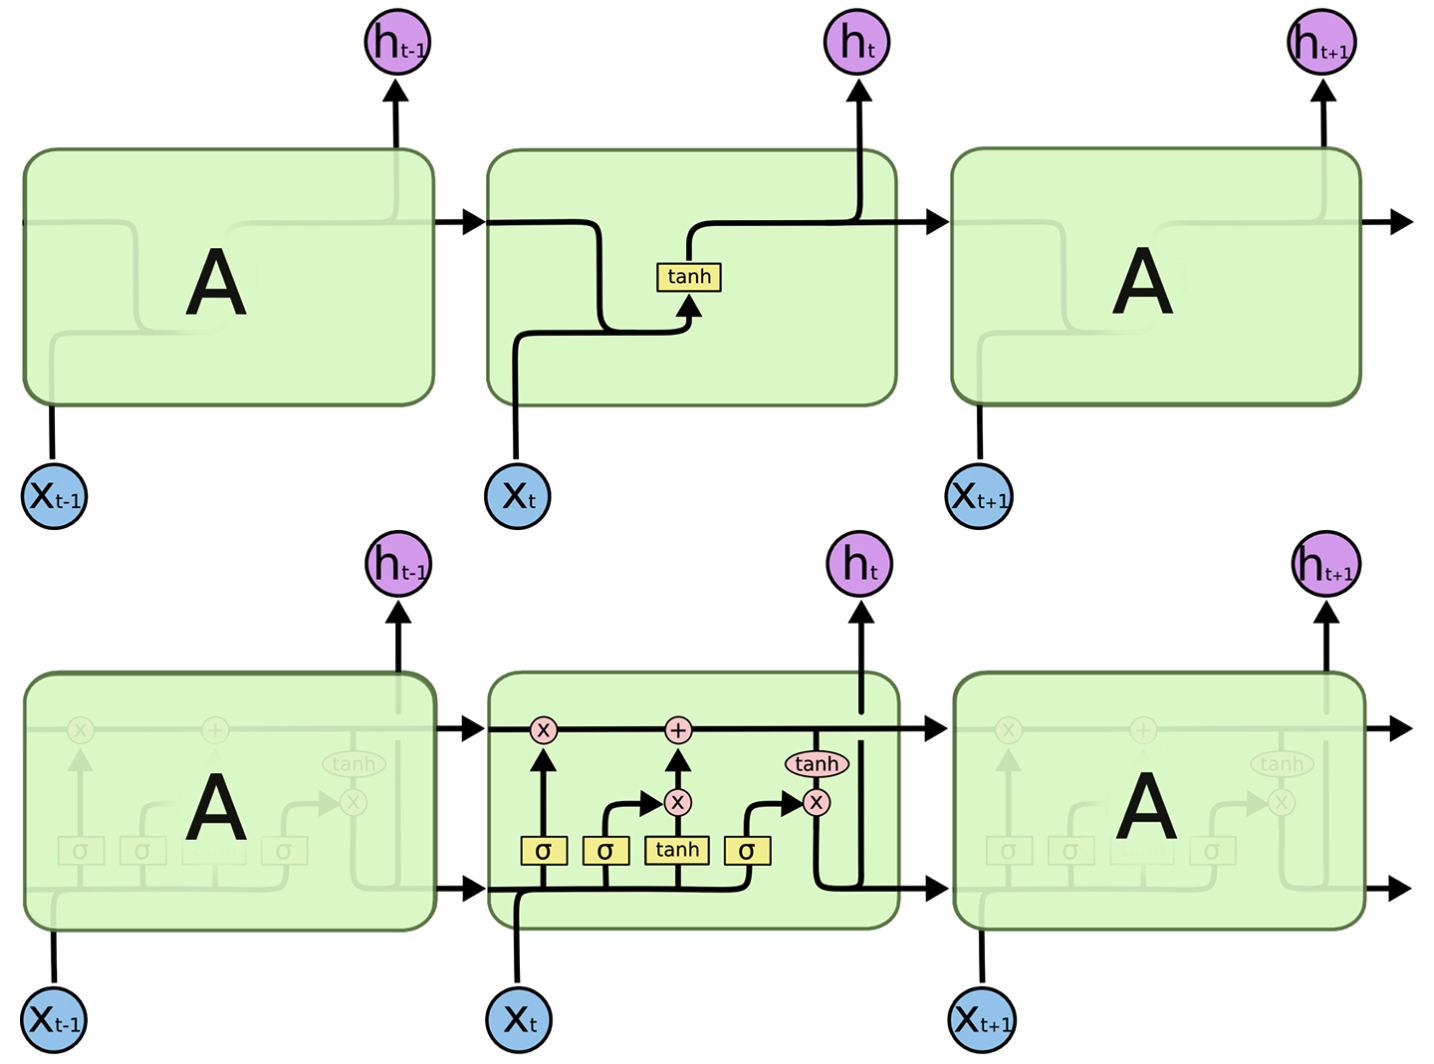
\includegraphics[scale = 0.15]{10.png}
	\caption{RNNs module structure vs. LSTM module structure}
\end{figure}
\noindent The key point of LSTM is that it includes a "coveyor belt" within the module structure. Information will transfer on this "conveyor belt" and only few linear interaction can prevent the loss of information. There are three different gates collaborate together : "Foget", "Refresh" and "Output". \\
\subsection{GRU}
\noindent When we train the LSTM module, we find that although the result comes from LSTM is much better than vallina RNN module, but the time cost is  higher. To reduce the training time, we use GRU model to replace LSTM model.
\begin{figure}[H]
	\centering
	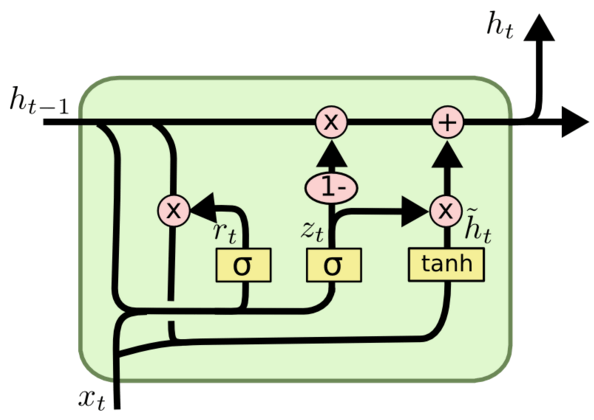
\includegraphics[scale = 0.15]{11.png}
	\caption{GRU module}
\end{figure}
\noindent It's obvious that inside of the GRU module, there are only two gates named "Refresh" and " Reset" instead of three gates in the LSTM module. The "Refresh" gate decides how much previous information we need to go through and the "Reset" gate decides how much former information the module should discard.\\

\noindent In theoretical, because of the decrease of parameters in the GRU module, the computational efficiency of GRU will higher than LSTM. \\
\subsection{ Attention}
\noindent The traditional Attention Mechanism is also called Soft Attention, which the hidden status of the encoded code is obtained through the deterministic score calculation. Besides, Soft Attention is parameterized, so it can be derived and can be embedded in the model and trained directly. Gradients can be back-propagated to other parts of the model through the Attention Mechanism module.\\
\begin{figure}[H]
	\centering
	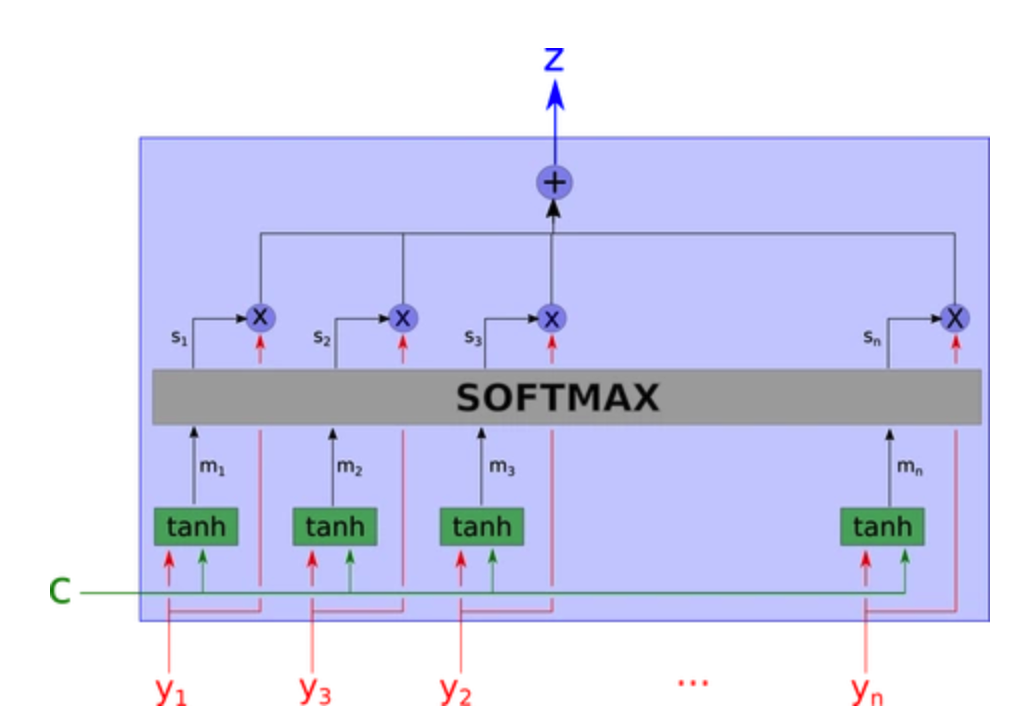
\includegraphics[scale = 0.15]{s1.png}
	\caption{ Attention module}
\end{figure}
\noindent Our model is inspired by this soft attention model. With LSTM inside the model, we put weights on the LSTM output and concatenate them to get final result.
\section{ Implementation}
\subsection{Embedding}
\noindent Before we feed the training data into our model, the first thing after cleaning the data is to transfer string type data to vectors. The dictionary we use to convert string is wiki-news-300d-1M.vec which supplied by Kaggle. Wiki-news-300d-1M is a dictionary with one million words(including punctuations and numbers). And each key is one word, each value is a 1-dimension  word vector with 300 numbers.\\

\noindent For the words in training data which can  be found in wiki-news-dictionary, we replace them with vectors. For those can’t be found in wiki-news-dictionary and also escaped from our preprocessing, we initialize them with a random vector which is based on the distribution of the words in text.\\
\begin{figure}[h]
	\centering
	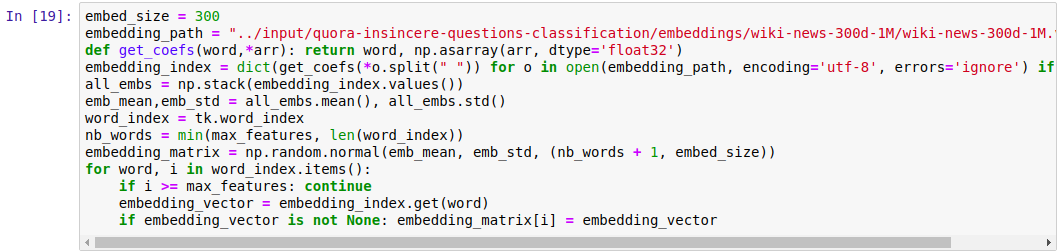
\includegraphics[scale = 0.2]{41.png}
	\caption{Initialize training dataset with random vector}
\end{figure}\\
\noindent After all these steps, the data is ready to be fed into our models.\\

\subsection{LSTM}
\subsubsection{One layer LSTM}
\begin{figure}[h]
	\centering
	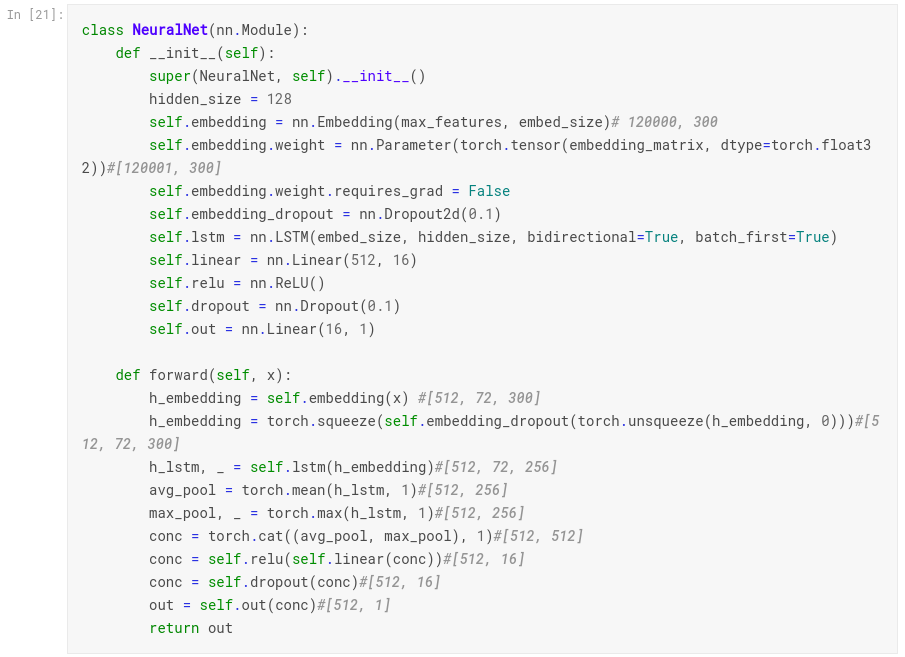
\includegraphics[scale = 0.2]{42.png}
	\caption{One layer LSTM model}
\end{figure}
\noindent First model is just a simple one-layer LSTM model, after going through the LSTM layer, the output of that layer goes through two separate pooling layers in order to obtain information as much as possible. Then we concatenate the two outputs of the pooling layers and put it into an activation layer and then dropout followed by a linear layer.\\

\noindent There’s only one hyperparameter we adjust in this project- number of epochs. In order to save time, we first tried 5, 7, 10 epochs to train our raw data without replacing misspelling words. The result is shown in Fig.23.\\
\begin{figure}[H]
	\centering
	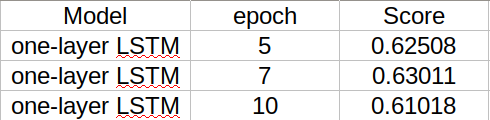
\includegraphics[scale = 0.2]{421.png}
	\caption{Different epochs with one-layer LSTM}
\end{figure}
\noindent Obviously, 7-epoch LSTM has the highest score. And this is the reason that we choose seven epochs to train our following models.
With preprocessed data fed into model, we get the result shown below. And the average time training one epoch is at around 75s.
\begin{figure}[H]
	\centering
	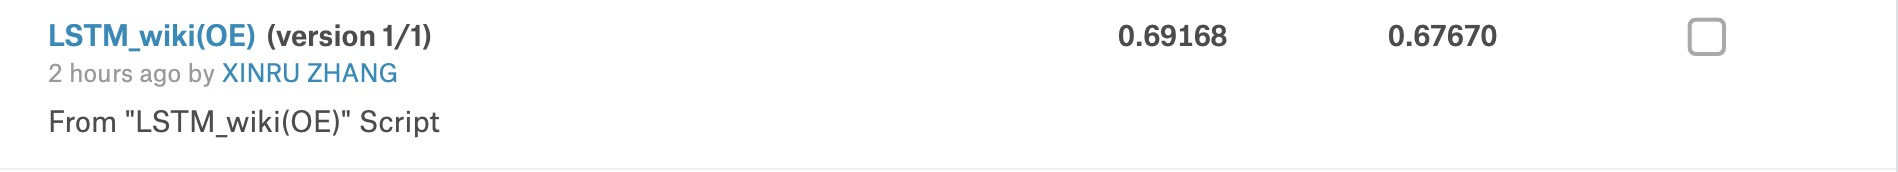
\includegraphics[scale = 0.2]{4211.jpeg}
	\caption{One-layer LSTM(7 epoch)
	}
\end{figure}
\begin{figure}[H]
	\centering
	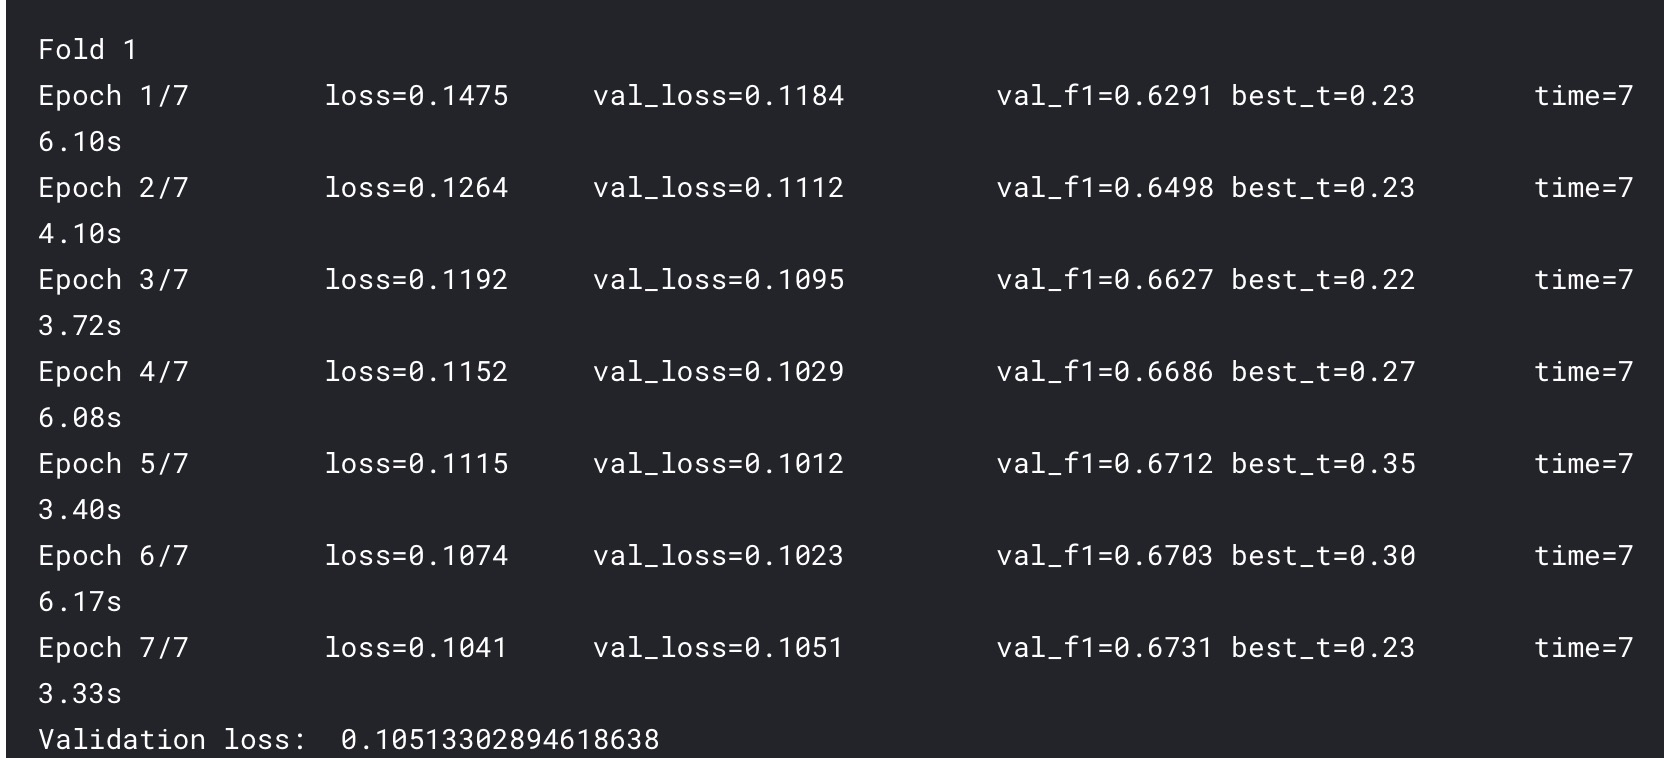
\includegraphics[scale = 0.2]{4212.jpeg}
	\caption{Part training result. Average training time consuming for one epoch is around 75 second
	}
\end{figure}
\subsubsection{ Two and three layers LSTM}
\noindent We also tried two - layer and three-layer LSTM models with seven epochs. With raw data, the two-layer LSTM got 0.63068 on final result which performs better than one-layer LSTM but the three-layer LSTM got 0.62601 which is worse than the two-layer LSTM model. The reason may be that three layers model is too much for the training data, the model got overfitting on the data.\\
\begin{figure}[H]
	\centering
	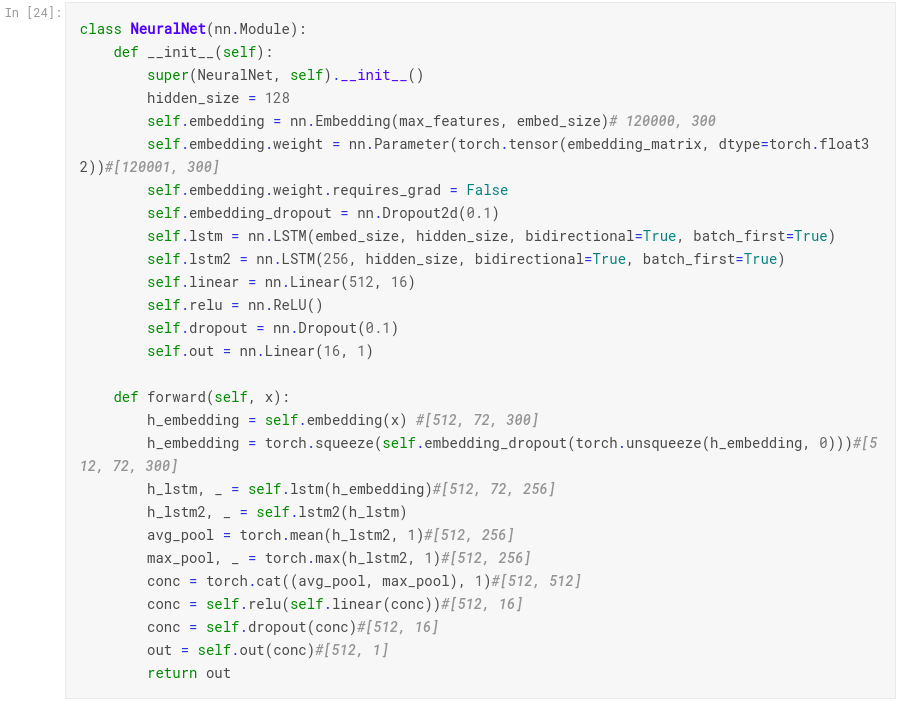
\includegraphics[scale = 0.2]{422.png}
	\caption{Two-layer LSTM}
\end{figure}
\noindent After feeding preprocessed data to two-layer LSTM model, we got 0.68421 which is the highest score among all the LSTM models.\\
	\begin{figure}[H]
		\centering
		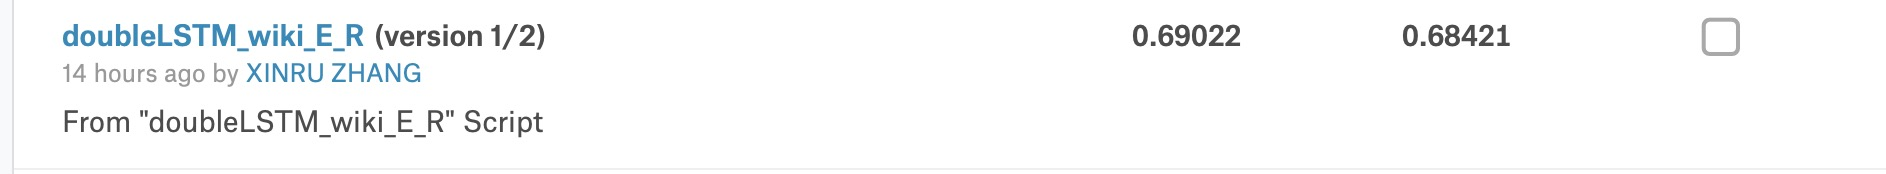
\includegraphics[scale = 0.2]{4221.jpeg}
		\caption{ Two-layer LSTM score }
	\end{figure}
\subsection{Simple GRU}
\noindent Simply replacing nn.LSTM with nn.GRU give us one-layer GRU model. Compared to one-layer LSTM, we got a higher score(0.68206) and less training time(at around 44s).\\
	\begin{figure}[H]
	\centering
	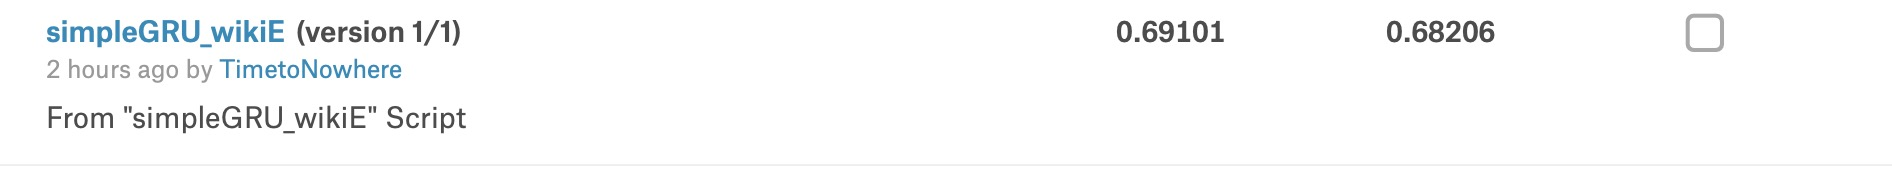
\includegraphics[scale = 0.2]{431.jpeg}
	\caption{ One-layer GRU socre}
\end{figure}
\begin{figure}[H]
	\centering
	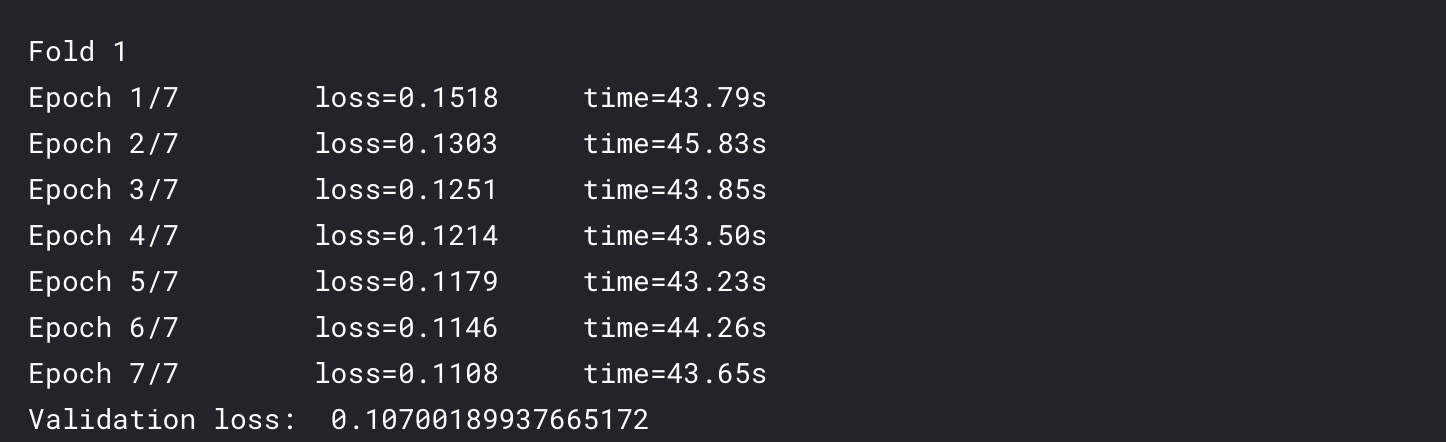
\includegraphics[scale = 0.2]{432.jpeg}
	\caption{Part training result. Average training time consuming for one epoch is around 44 second}
\end{figure}
\subsection{Attention}
\noindent The structure of attention model is shown below. The score we got is 0.68506 which is the highest score we have.\\
\begin{figure}[H]
	\centering
	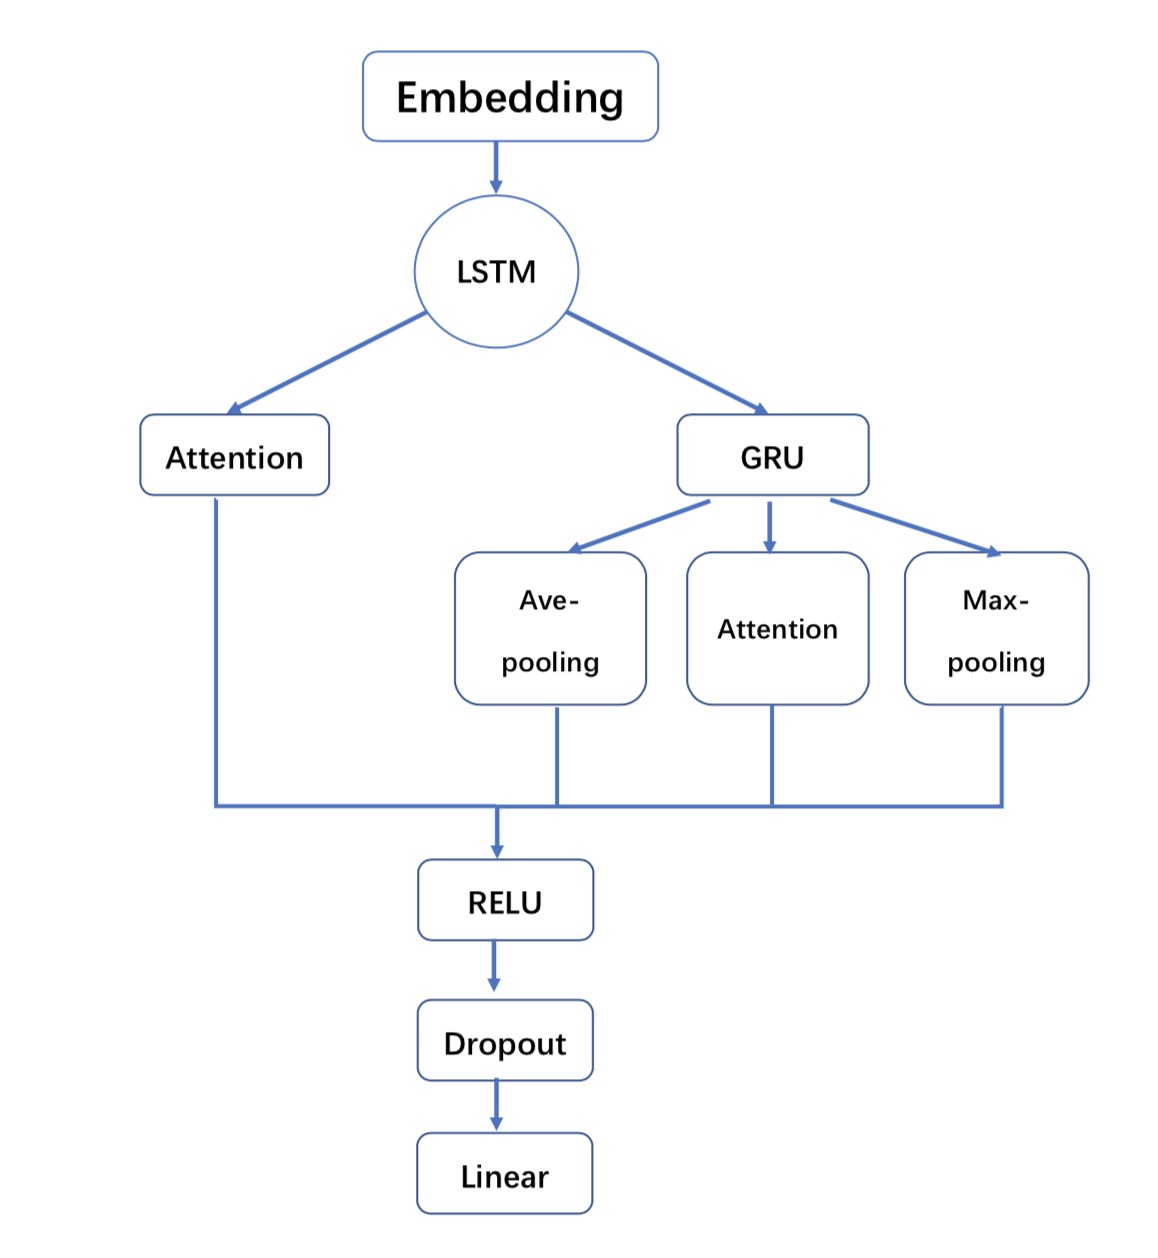
\includegraphics[scale = 0.2]{442.jpeg}
	\caption{Attention mode}
\end{figure}
\noindent In the Fig.31, we add two weights matrix at the attention step. In training data, not all words’ contributions are the same. The intuition to use attention model is to let model pay more attention on some ‘useful’ words instead of treat every word equally.\\
\begin{figure}[H]
	\centering
	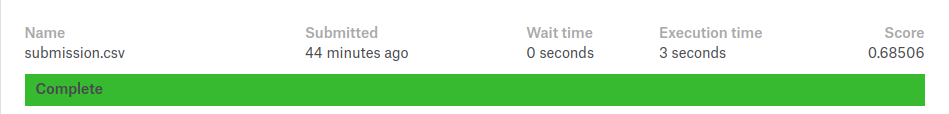
\includegraphics[scale = 0.2]{441.png}
	\caption{Attention model score}
\end{figure}

\section*{Reference}
\small

\noindent [1] Goodfellow, I.\ \& Bengio, Y.\ \& Courville, A.\ (2016) Deep Learning. {\it Modern Practical Deep Networks},
pp.\ 367--403. Cambridge, MA: MIT Press.\\

\noindent[2] Supervise, ly., (2017) Towards Data Science:
{\it Evolution: from vanilla RNN to LSTM \& GRU.} [online]Available at <https://towardsdatascience.com/lecture-evolution-from-vanilla-rnn-to-gru-lstms> (02/12/2019 12:14)\\

\noindent[3] Hoffman, G.(2018). {\it Introduction to LSTMs with Pytorch.} O'Reilly AI Newsletter, 54, 66-80.\\

\noindent[4] Adrianna, X., (2017) More or Less?:{\it Talking about the difference with LSTM and GRU.}
[online]Available at <https://blog.csdn.net/u012223913/article/details/77724621> (30/11/2019 17:34)\\

\noindent[5]  Hao, L., (2018) Talking about Nature Language Processing: {\it
Word Embedding}. [online]Available at <https://blog.csdn.net/L\_R\_H000/article/details/81320286> (02/12/2019 12:44)\\

\noindent[6]  Xiaozhou, Y. \ \& Feifei, T.\ \& Rongzhi, Q. (2016). {\it Improvement of activation function in recurrent neuron network.} Journal of computer and modernization,12, 14-27.\\

\noindent[7] Zafarali, A.(Jun 29, 2017). How to Visualize Your Recurrent Neural Network with Attention in Keras. {\it Medium website}
\end{document}
